\documentclass[conference]{IEEEtran}


% *** GRAPHICS RELATED PACKAGES ***
%
\ifCLASSINFOpdf
  % \usepackage[pdftex]{graphicx}
  % declare the path(s) where your graphic files are
  % \graphicspath{{../pdf/}{../jpeg/}}
  % and their extensions so you won't have to specify these with
  % every instance of \includegraphics
  % \DeclareGraphicsExtensions{.pdf,.jpeg,.png}
\else
  % or other class option (dvipsone, dvipdf, if not using dvips). graphicx
  % will default to the driver specified in the system graphics.cfg if no
  % driver is specified.
  % \usepackage[dvips]{graphicx}
  % declare the path(s) where your graphic files are
  % \graphicspath{{../eps/}}
  % and their extensions so you won't have to specify these with
  % every instance of \includegraphics
  % \DeclareGraphicsExtensions{.eps}
\fi
% graphicx was written by David Carlisle and Sebastian Rahtz. It is
% required if you want graphics, photos, etc. graphicx.sty is already
% installed on most LaTeX systems. The latest version and documentation
% can be obtained at:
% http://www.ctan.org/pkg/graphicx
% Another good source of documentation is "Using Imported Graphics in
% LaTeX2e" by Keith Reckdahl which can be found at:
% http://www.ctan.org/pkg/epslatex
%
% latex, and pdflatex in dvi mode, support graphics in encapsulated
% postscript (.eps) format. pdflatex in pdf mode supports graphics
% in .pdf, .jpeg, .png and .mps (metapost) formats. Users should ensure
% that all non-photo figures use a vector format (.eps, .pdf, .mps) and
% not a bitmapped formats (.jpeg, .png). The IEEE frowns on bitmapped formats
% which can result in "jaggedy"/blurry rendering of lines and letters as
% well as large increases in file sizes.
%
% You can find documentation about the pdfTeX application at:
% http://www.tug.org/applications/pdftex





% *** MATH PACKAGES ***
%
%\usepackage{amsmath}
% A popular package from the American Mathematical Society that provides
% many useful and powerful commands for dealing with mathematics.
%
% Note that the amsmath package sets \interdisplaylinepenalty to 10000
% thus preventing page breaks from occurring within multiline equations. Use:
%\interdisplaylinepenalty=2500
% after loading amsmath to restore such page breaks as IEEEtran.cls normally
% does. amsmath.sty is already installed on most LaTeX systems. The latest
% version and documentation can be obtained at:
% http://www.ctan.org/pkg/amsmath





% *** SPECIALIZED LIST PACKAGES ***
%
%\usepackage{algorithmic}
% algorithmic.sty was written by Peter Williams and Rogerio Brito.
% This package provides an algorithmic environment fo describing algorithms.
% You can use the algorithmic environment in-text or within a figure
% environment to provide for a floating algorithm. Do NOT use the algorithm
% floating environment provided by algorithm.sty (by the same authors) or
% algorithm2e.sty (by Christophe Fiorio) as the IEEE does not use dedicated
% algorithm float types and packages that provide these will not provide
% correct IEEE style captions. The latest version and documentation of
% algorithmic.sty can be obtained at:
% http://www.ctan.org/pkg/algorithms
% Also of interest may be the (relatively newer and more customizable)
% algorithmicx.sty package by Szasz Janos:
% http://www.ctan.org/pkg/algorithmicx




% *** ALIGNMENT PACKAGES ***
%
%\usepackage{array}
% Frank Mittelbach's and David Carlisle's array.sty patches and improves
% the standard LaTeX2e array and tabular environments to provide better
% appearance and additional user controls. As the default LaTeX2e table
% generation code is lacking to the point of almost being broken with
% respect to the quality of the end results, all users are strongly
% advised to use an enhanced (at the very least that provided by array.sty)
% set of table tools. array.sty is already installed on most systems. The
% latest version and documentation can be obtained at:
% http://www.ctan.org/pkg/array


% IEEEtran contains the IEEEeqnarray family of commands that can be used to
% generate multiline equations as well as matrices, tables, etc., of high
% quality.




% *** SUBFIGURE PACKAGES ***
%\ifCLASSOPTIONcompsoc
%  \usepackage[caption=false,font=normalsize,labelfont=sf,textfont=sf]{subfig}
%\else
%  \usepackage[caption=false,font=footnotesize]{subfig}
%\fi
% subfig.sty, written by Steven Douglas Cochran, is the modern replacement
% for subfigure.sty, the latter of which is no longer maintained and is
% incompatible with some LaTeX packages including fixltx2e. However,
% subfig.sty requires and automatically loads Axel Sommerfeldt's caption.sty
% which will override IEEEtran.cls' handling of captions and this will result
% in non-IEEE style figure/table captions. To prevent this problem, be sure
% and invoke subfig.sty's "caption=false" package option (available since
% subfig.sty version 1.3, 2005/06/28) as this is will preserve IEEEtran.cls
% handling of captions.
% Note that the Computer Society format requires a larger sans serif font
% than the serif footnote size font used in traditional IEEE formatting
% and thus the need to invoke different subfig.sty package options depending
% on whether compsoc mode has been enabled.
%
% The latest version and documentation of subfig.sty can be obtained at:
% http://www.ctan.org/pkg/subfig




% *** FLOAT PACKAGES ***
%
%\usepackage{fixltx2e}
% fixltx2e, the successor to the earlier fix2col.sty, was written by
% Frank Mittelbach and David Carlisle. This package corrects a few problems
% in the LaTeX2e kernel, the most notable of which is that in current
% LaTeX2e releases, the ordering of single and double column floats is not
% guaranteed to be preserved. Thus, an unpatched LaTeX2e can allow a
% single column figure to be placed prior to an earlier double column
% figure.
% Be aware that LaTeX2e kernels dated 2015 and later have fixltx2e.sty's
% corrections already built into the system in which case a warning will
% be issued if an attempt is made to load fixltx2e.sty as it is no longer
% needed.
% The latest version and documentation can be found at:
% http://www.ctan.org/pkg/fixltx2e


%\usepackage{stfloats}
% stfloats.sty was written by Sigitas Tolusis. This package gives LaTeX2e
% the ability to do double column floats at the bottom of the page as well
% as the top. (e.g., "\begin{figure*}[!b]" is not normally possible in
% LaTeX2e). It also provides a command:
%\fnbelowfloat
% to enable the placement of footnotes below bottom floats (the standard
% LaTeX2e kernel puts them above bottom floats). This is an invasive package
% which rewrites many portions of the LaTeX2e float routines. It may not work
% with other packages that modify the LaTeX2e float routines. The latest
% version and documentation can be obtained at:
% http://www.ctan.org/pkg/stfloats
% Do not use the stfloats baselinefloat ability as the IEEE does not allow
% \baselineskip to stretch. Authors submitting work to the IEEE should note
% that the IEEE rarely uses double column equations and that authors should try
% to avoid such use. Do not be tempted to use the cuted.sty or midfloat.sty
% packages (also by Sigitas Tolusis) as the IEEE does not format its papers in
% such ways.
% Do not attempt to use stfloats with fixltx2e as they are incompatible.
% Instead, use Morten Hogholm'a dblfloatfix which combines the features
% of both fixltx2e and stfloats:
%
% \usepackage{dblfloatfix}
% The latest version can be found at:
% http://www.ctan.org/pkg/dblfloatfix




% *** PDF, URL AND HYPERLINK PACKAGES ***
%
%\usepackage{url}
% url.sty was written by Donald Arseneau. It provides better support for
% handling and breaking URLs. url.sty is already installed on most LaTeX
% systems. The latest version and documentation can be obtained at:
% http://www.ctan.org/pkg/url
% Basically, \url{my_url_here}.




% *** Do not adjust lengths that control margins, column widths, etc. ***
% *** Do not use packages that alter fonts (such as pslatex).         ***
% There should be no need to do such things with IEEEtran.cls V1.6 and later.
% (Unless specifically asked to do so by the journal or conference you plan
% to submit to, of course. )

\usepackage{graphicx}

% correct bad hyphenation here
\hyphenation{op-tical net-works semi-conduc-tor}


\begin{document}
%
% paper title
% Titles are generally capitalized except for words such as a, an, and, as,
% at, but, by, for, in, nor, of, on, or, the, to and up, which are usually
% not capitalized unless they are the first or last word of the title.
% Linebreaks \\ can be used within to get better formatting as desired.
% Do not put math or special symbols in the title.
\title{Fusion of Music Styles Using LSTM Recurrent Neural Networks}


% author names and affiliations
% use a multiple column layout for up to three different
% affiliations
\author{\IEEEauthorblockN{Harsh Lal}
\IEEEauthorblockA{
UCSD(CSE)\\
PID: A53244610\\
Email: hlal@ucsd.edu}
\and
\IEEEauthorblockN{Jacob Sundstrom}
\IEEEauthorblockA{
UCSD(Music)\\
PID: A09060631\\
Email: jlsundst@ucsd.edu}
\and
\IEEEauthorblockN{Nakul Tiruviluamala}
\IEEEauthorblockA{
UCSD(Music)\\
PID: FILLHERE\\
Email: ntiruvil@ucsd.edu}
\and
\IEEEauthorblockN{David Defilippo}
\IEEEauthorblockA{
UCSD(Music)\\
PID: FILLHERE\\
Email: ddefilip@ucsd.edu}}

% conference papers do not typically use \thanks and this command
% is locked out in conference mode. If really needed, such as for
% the acknowledgment of grants, issue a \IEEEoverridecommandlockouts
% after \documentclass

% for over three affiliations, or if they all won't fit within the width
% of the page, use this alternative format:
%
%\author{\IEEEauthorblockN{Michael Shell\IEEEauthorrefmark{1},
%Homer Simpson\IEEEauthorrefmark{2},
%James Kirk\IEEEauthorrefmark{3},
%Montgomery Scott\IEEEauthorrefmark{3} and
%Eldon Tyrell\IEEEauthorrefmark{4}}
%\IEEEauthorblockA{\IEEEauthorrefmark{1}School of Electrical and Computer Engineering\\
%Georgia Institute of Technology,
%Atlanta, Georgia 30332--0250\\ Email: see http://www.michaelshell.org/contact.html}
%\IEEEauthorblockA{\IEEEauthorrefmark{2}Twentieth Century Fox, Springfield, USA\\
%Email: homer@thesimpsons.com}
%\IEEEauthorblockA{\IEEEauthorrefmark{3}Starfleet Academy, San Francisco, California 96678-2391\\
%Telephone: (800) 555--1212, Fax: (888) 555--1212}
%\IEEEauthorblockA{\IEEEauthorrefmark{4}Tyrell Inc., 123 Replicant Street, Los Angeles, California 90210--4321}}




% use for special paper notices
%\IEEEspecialpapernotice{(Invited Paper)}




% make the title area
\maketitle

% As a general rule, do not put math, special symbols or citations
% in the abstract
\begin{abstract}
Appeal of a musical composition is almost exclusively subjective in that it is a combination of the tastes, preferences, and history of an individual's experiences. That is, it is perceived and judged qualitatively in a different way by different individuals. In this project we propose to build a deep learning system which could take $n$ different samples of a jazz soloist - especially a variety of samples of specific 'styles' - and generate sound using current input as well as feedback and memory from the past samples. This generation can then be judged by a 'human' agent and the parameters of the neural network could be adjusted accordingly to generate a fusion music that is more closer and appealing to agent's expectations. Recurrent neural networks with Long Short Term Memory (LSTMs) in particular have shown promise as a module that can learn long songs sequences, and generate new compositions based on the song's harmonic structure and the feedback inherent in the network. \cite{judy2} We plan to explore the same through our experiments.
\end{abstract}

% no keywords




% For peer review papers, you can put extra information on the cover
% page as needed:
% \ifCLASSOPTIONpeerreview
% \begin{center} \bfseries EDICS Category: 3-BBND \end{center}
% \fi
%
% For peerreview papers, this IEEEtran command inserts a page break and
% creates the second title. It will be ignored for other modes.
\IEEEpeerreviewmaketitle



\section{Introduction}
% no \IEEEPARstart
Music is an extraordinarily appealing auditory sensation and the classification of musical style can be virtually infinite. Since the dawn of music there has been a desire to fuse musical styles in different ways, taking either essential or superficial musical aspects of two or more compositions or performers. Usually highly skilled musicians mix different musical styles and compositions intuitively, creating a fusion of style that they themselves are satisfied with. In this work, we we try to combine different musical styles using deep learning techniques. All of the current work is performed using MIDI files but can be easily extended to incorporate new formats. It should be noted, moreover, that musical style is used in a broad sense in that individual players within a single genre can have differing "styles".\\

The most straightforward way to generate music with with a recurrent neural network (RNN) is to use the network as a single step predictor. The network can be trained to predict notes at time $t+1$ conditioned on notes till time $t$ as inputs. After the training is completed, the network can be seeded with random initial inputs (mostly from training samples) to generate novel musical compositions using subsequent output generated as input for next generation. This note-by note approach was first examined by Bharucha \& Todd.\cite{todd,eck}\\

A generic feed-forward neural network would not be a good fit at composing music using the technique described above. The main reason behind this is the inability to memorize any information about the past, thereby not being able to keep track of variations \& periodicity of a song's  feature across time. In principle RNN does not suffer this limitation owing to its recurrent connections and hidden activation layers that may act memory elements, thereby exhibiting temporal behaviour. However they do not perform well at the task of modelling long duration temporal dynamics as studied by Mozer.\cite{mozer}, with most likely cause being the the problem of vanishing gradients associated with RNNs.\cite{hochreiter}\\

So we explore the viability of using LSTM recurrent neural networks for the same and experiment with fusion of different musical styles. For this we extract features like notes, rhythm and amplitude from midi files as described in \ref{Feature Engineering}. We then pre-process it and pass it to a neural network. We train neural networks separately for each of the features. We then generate the chosen features from target musical style and then combine them to generate the final output result as described in \ref{Model description}. We then experiment with varying styles and describe out results in latter sections.

\section{Dataset}
The most important considerations in choosing a dataset were both musical and practical. Musically, the dataset had to be interesting enough to\\

The choice to use MIDI files as our dataset file was one of practical considerations. Sound files, such as MP3 and WAV, capture the waveform of the sound and reproduce the sound as it was recorded or synthesized. The waveform itself contains no musically meaningful material without extensive processing, beat tracking, onset detection, frequency analysis, etc. Moreover, the analysis and extraction methods used on signals is often imprecise and typically of an entire song with all instruments playing simultaneously. Extracting a single instrument from the texture and then accurately representing it quantitatively is extraordinarily difficult and creates additional difficulties of representing that information in a musically meaningful fashion.\\

The dataset consists of transcribed jazz solos as found on the Jazzomat Research Project. Jazz as a genre offered several advantages: specific soloists often have repeated rhythmic and harmonic ideas that carry through different songs, jazz standards offered a predictable harmonic palette with which to use, and transcribed jazz solos are often available for free. Additionally, the solos that were chosen were those of monophonic instruments, like that of the saxophone or trumpet and unlike that of the piano or guitar, since these instruments play one note at a time. This made the extraction of rhythmic data immensely easier and less complicated.\\

In order to facilitate the largest datasets and given the stylistic choices specific to certain soloists, the files were grouped by soloist. This allowed us to easily maintain a repository for the harmonic, rhythmic, and dynamic information of a given soloist.\\ 

There are, of course, certain caveats. Jazz standards, as a general principle, change key throughout the course of the tune. While this is fixed, the MIDI file format makes parsing this information on a temporal basis extremely difficult. It was therefore not including in the the final form of the pre-processed data.

\subsection{Preprocessing}
<<<<<<< HEAD
The biggest challenge of preprocessing was to somehow maintain the musical integrity of the data we extracted. This particular challenge proved to be too difficult to grapple with in the time allotted and the choice was made to simple normalize the data to render them song agnostic. That is, the representation of the data was not dependent on either the key, tempo, or other musical feature of the specific song. Within the MIDI file itself, 'note' events, such as note-on and note-off govern the resulting sound and it is from these note events that features were extracted.
=======
The biggest challenge of pre-processing was to somehow maintain the musical integrity of the data we extracted. This particular challenge proved to be too difficult to grapple with in the time allotted and the choice was made to simple normalize the data to render them song agnostic. That is, the representation of the data was not dependent on either the key, tempo, or other musical feature of the specific song. Within the MIDI file itself, 'note' events, such as note-on and note-off govern the resulting sound and it is from these note events that features were extracted.\\

Pre-processing was done in two steps. First, from each individual MIDI file notes, rhythm, and velocities (amplitudes of notes) were extracted. Note and velocity information is extracted in a straightforward manner as the file contains these values directly. Rhythm, however, is prescribed indirectly through what are called 'note-on' and 'note-off' events that tell the MIDI engine when a note of a given pitch and velocity is to begin and when it is to end. This is further complicated by the fact that time in a MIDI file is given in ticks per beat, the value of which can vary across different MIDI files to give greater or lesser temporal resolution, and each note event is prescribed a delta time value, which is the number ticks that have elapsed since the most recent message. From the delta time value of a given note-off event and its corresponding note-on event, the duration, in ticks per beat, could be calculated. These values were then normalized such that they became tempo and ticks per beat agnostic. The result is a duration of a note that was a ratio of the ticks per beat value. The same type of normalization occurred with notes, as well. All of the solos were transposed to the key of C, regardless of their original key. The notes were then further normalized into intervals of semitones thereby increasing the key indifference of the data.\\

It is common knowledge that music is not a steady stream of sound; rather, it is comprised of both sound and silence. However, while it was fairly trivial to include rests in the pre-processed rhythmic data, the results from said data were unusable in a musically meaningful way. Therefore, the choice was made to not include rests in the data and thus, not include rests in the generated rhythmic data. This is an obstacle that would be needed to overcome in further iterations.
>>>>>>> 590597e916c9e8a9c2fd4701bc7a7d9a12a13d22

\subsection{Feature Engineering} \label{Feature Engineering}
Musical features are numerous and, depending on what one is seeking, can take many forms. In our case, we sought the most simple and basic traditional musical features: pitch, rhythm, and dynamic (or amplitude). The structure of MIDI files is such that these three features are prominently and clearly encoded. In a sound file that represents a waveform, extracting pitch information takes for form of FFT analysis which is then translated to musical pitch. This processes is difficult to manage and can introduce rounding errors, not to mention the difficulties with extracting a single instrument from a song texture. Moreover, re synthesizing such analysis extracted features into a sound file is riddled with additional challenges. Although one might be able to extract a pitch of an instrument, this says nothing about envelope characteristics, instrumental timbre, or accurate rhythmic representation. Thus, analyzing a sound file did not meet the ease-of-use criteria of our data.\\

MIDI files, on the other hand, contain in an easy to read format all the salient features we wanted access to in addition to being simple to parse. MIDI files are organized into 'tracks' which contain a single instrument, not necessarily monophonic. Additionally, a 'note' in MIDI-space is defined by two events: a 'note-on' and a 'note-off' that tell the MIDI engine when to start a note and when to terminate it. Each event contains three pieces of information: pitch, velocity, and delta time, which is the time elapsed between the last MIDI event and this event. Specifics on the extraction of pitch, rhythm, and amplitude are in sections \ref{f1pitch}, \ref{f2rhythm}, and \ref{f3amplitude}, respectively. The important thing to note, however, is that the the data of each feature of a particular player's repertoire was concatenated into a single set, such that all of player $p$'s harmonic information is contained in one set, all of their rhythmic information in another, and all the amplitude information in a third.\\

<<<<<<< HEAD
\subsubsection{Feature 1: Pitch} \label{f1pitch}
Extraction of pitch information from a MIDI file is fairly straightforward. Since each 'note' is comprised of two messages that give pitch, it is simple to extract the pitch information from a note-on event. MIDI notes exist in the range between 0 and 127, each number representing a single pitch in 12-tone equal temperament with 60 being middle C. In other words, each MIDI pitch number corresponds to a single key on the piano but extends beyond the piano range in both directions.
=======
\subsubsection{Feature 1:Pitch} \label{f1pitch}
Extraction of pitch information from a MIDI file is fairly straightforward. Since each 'note' is comprised of two messages that give pitch, it is simple to extract the pitch information from a note-on event. MIDI notes exist in the range between 0 and 127, each number representing a single pitch in 12-tone equal temperament with 60 being middle C. In other words, each MIDI pitch number corresponds to a single key on the piano but extends beyond the piano range in both directions.\\
>>>>>>> 590597e916c9e8a9c2fd4701bc7a7d9a12a13d22

For a given song, the entire track containing the desired instrument is parsed and pitches are saved in an array in the order in which they appear in the solo. Since a MIDI file also contains key information, each song was transposed to the key of C (harmonic changes throughout the song notwithstanding). The pitch sequences were then converted to sequences of semitone intervals to further refine the pitch information and render it harmony-agnostic resulting in an array of intervals that is the length of the number of notes in the song minus one. Extracting, combining, and normalizing the notes in this way - that is, apart from harmony - rendered any notion of harmonic progression null. Even if an entire network were trained on one players repertoire on a single set of harmonic changes, it was not possible to keep track of these changes in the order they occur in the song when sampling the model.\\

This process was repeated for each song of a particular player's solo in the dataset. The resulting interval sequences were then appended together to give a long sequence of intervals that is the length of the sum of all the notes in all the solos in the dataset minus the number of songs in that particular players' set of songs.\\

<<<<<<< HEAD
\subsubsection{Feature 2: Rhythm} \label{f2rhythm}
Rhythmic information can be deduced in a MIDI file by examing the delta time values of sequenctial MIDI events. Each MIDI message contains a time value (better understood as delta time) which is the time in ticks per beat that elapsed between the previous event and this event. That is, if a MIDI message contains a time value of 100, we know that this event or message occurs 100 ticks after the previous message. Using this information, it is relatively trivial to deduce the duration of a note or rest when complementary note-on and note-off events can be found. To be sure, if a note-on event of pitch $p$ occurs at time $t$ and the complementary note-off event occurs with a delta time value of 100, we know that the length of the note of pitch $p$ is 100 ticks long.
=======
\subsubsection{Feature 2:Rhythm} \label{f2rhythm}
Rhythmic information can be deduced in a MIDI file by examining the delta time values of sequential MIDI events. Each MIDI message contains a time value (better understood as delta time) which is the time in ticks per beat that elapsed between the previous event and this event. That is, if a MIDI message contains a time value of 100, we know that this event or message occurs 100 ticks after the previous message. Using this information, it is relatively trivial to deduce the duration of a note or rest when complementary note-on and note-off events can be found. To be sure, if a note-on event of pitch $p$ occurs at time $t$ and the complementary note-off event occurs with a delta time value of 100, we know that the length of the note of pitch $p$ is 100 ticks long.\\
>>>>>>> 590597e916c9e8a9c2fd4701bc7a7d9a12a13d22

In an important deviation from standard musical practice, the datasets did not include rests, or silences in a musical line. It is common knowledge that music is not a steady stream of sound; rather, it is comprised of both sound and silence. However, while it was fairly trivial to include rests in the pre-processed rhythmic data, the results from said data were unusable in a musically meaningful way. Therefore, the choice was made to not include rests in the data and thus, not include rests in the generated rhythmic data. This is an obstacle that would be needed to overcome in further iterations.\\

Once rhythms were reduced to ticks, the next step was to convert these values to fractions of a beat. The ticks per beat value in a MIDI file varies across different files depending on the time resolution needed for a particular song. Given that fact, the particular value of ticks per beat in a given song could not be relied upon to be consistent between and among different files. Thus, each delta time which represented rhythm was divided by the ticks per beat value in its respective file, giving a ratio of a beat that becomes tempo and ticks per beat agnostic. This allows the network to be training on musically more meaningful information as opposed to literal time as measured in milliseconds. In the same way pitch information was gathered, the rhythmic data of each song was concatenated to create a large set of rhythmic information of a particular player, independent of tempo, literal time, and ticks per beat.\\

<<<<<<< HEAD
\subsubsection{Feature 3: Amplitude} \label{f3amplitude}
In MIDI-space, amplitude is called velocity and is given as a value between 0 and 127. 0 is essentially silent while 127 is the maximum amplitude. Important to note is that unlike a real instrument, different amplitudes do not change the spectral or timbral charactaristics of the sound. It is merely softer or louder without the sound quality being different in any way. In a real instrument, for instance, playing softer often reduces the presence of high frequency harmonics while the MIDI sound contains the same harmonic profile whether it is loud or soft.
=======
\subsubsection{Feature 3:Amplitude} \label{f3amplitude}
In MIDI-space, amplitude is called velocity and is given as a value between 0 and 127. 0 is essentially silent while 127 is the maximum amplitude. Important to note is that unlike a real instrument, different amplitudes do not change the spectral or timbral characteristics of the sound. It is merely softer or louder without the sound quality being different in any way. In a real instrument, for instance, playing softer often reduces the presence of high frequency harmonics while the MIDI sound contains the same harmonic profile whether it is loud or soft.\\
>>>>>>> 590597e916c9e8a9c2fd4701bc7a7d9a12a13d22

Velocities, then, are also part of the note events. For a note-off event, they are always 127 while the velocity value of note-on event determines the actual amplitude of the note. In the same way pitch was extracted from note-on event, velocity too was extracted from the same events. Moreover, since the velocity value is independent of both harmony and rhythm, there was no need to normalize the data since it is, in a sense, already normalized. Like \ref{f1pitch} and \ref{f2rhythm}, the resulting velocities were concatenated into a single set comprising the entirety of the velocities of a particular player's repertoire.

\section{Basic Architecture}
Feed-forward neural networks consists of 2 or more layers of processing units, each with weighted connection to the next layer. Each unit passes the sum of its weighted inputs through a non linear sigmoid function. Each layer's outputs are fed forward through the network to the next layer, until the output layer is reached. Weights are initialized to small initial random values. Via the back-propagation algorithm, outputs are compared to targets, and the errors are propagated back through the connection weights. Weights are updated by gradient descent. Through an iterative training procedure, examples(inputs) and targets are presented repeatedly; the network learns nonlinear function of the inputs. We explore these networks for the purpose of processing musical features.\cite{judy1}

\subsection{Recurrent Neural Networks}
Recurrent neural network (RNN) is a class of artificial neural network where connections between units form a directed cycle. This allows it to exhibit dynamic temporal behavior. Unlike feed-forward neural networks, RNNs can use their internal memory to process arbitrary sequences of inputs. These networks use shared parameters across time, thereby providing these networks with capability to remember time history.\\

A recurrent network uses feedback from one or more of its units as input in choosing the next output. This means that values generated by units at time step $t-1$, say $y(t-1)$, are part of the inputs $x(t)$ used in selecting the next set of outputs $y(t)$. A network maybe fully recurrent; that is all units are connected back to each other and to themselves. Or part of the network may be fed back in recurrent links. \cite{judy1}\\

\begin{figure}[h]
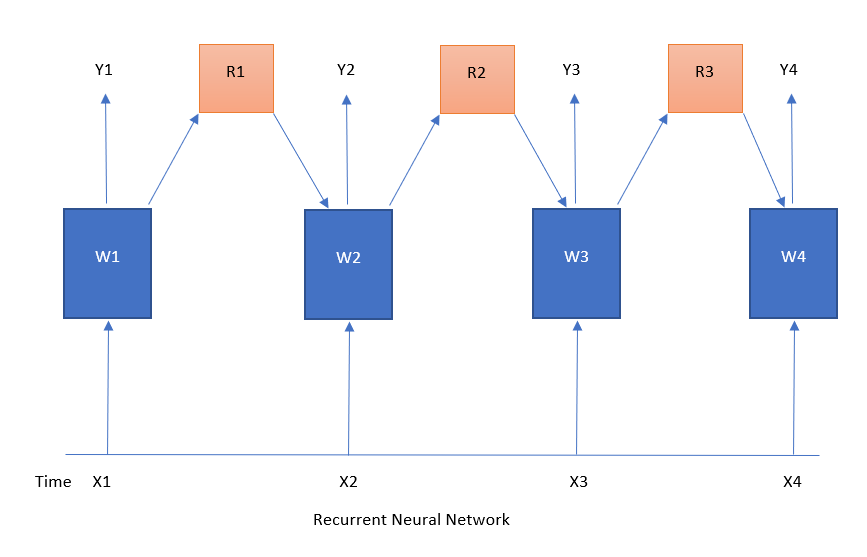
\includegraphics[width=0.5\textwidth]{1.PNG}
\caption{Basic Recurrent Neural Networks}
\label{fig:figure7}
\end{figure}

Figure \ref{fig:figure7} shows a typical RNN. Here if the sequence is stationary then the network simplifies where weights simplifies as $W = W1 = W2 = W3 = W4$ and recurrent connections simplifies as $R = R1 = R2 = R3$.
In recurrent neural networks we need to back propagate through time. Due to a lot of correlated updates per iteration may cause the problem of exploding or vanishing gradients. The problem of vanishing gradient is solved using LSTM (long short term memory) cells instead of regular neurons as is described in next section.

\subsection{LSTM}
Long Short-Term Memory (LSTM) is a recurrent neural network (RNN) architecture that has been designed to address the vanishing and exploding gradient problems of conventional RNNs. Unlike feed-forward neural networks, RNNs have cyclic connections making them powerful for modeling sequences. They have been successfully used for sequence labeling and sequence prediction tasks, such as handwriting recognition, language modeling, phonetic labeling of acoustic frames. \cite{lstm}\\
The LSTM network is a significant departure from other networks in that it uses hidden layer of memory blocks that can be thought of a complex processing units as shown in figure \ref{fig:figure1}. Departing from typical notion of neuron units that sums its weighted inputs and passes them to a non linear sigmoid function, each LSTM memory block contains gating units. The Write gate learns to controls when inputs are allowed to pass in to the cell, the Read gate learns to controls when cell's outputs are passed out of the block, and the Forget gate learns to control when to reset the memory.\\
\\The weight updates for each block of the LSTM network are complex because of the use of the $n$ memory cells and the three gates (described above) that control these $n$ cells within each block. Over and above each output unit of the whole network has a set of weights used to multiply the values coming from the memory blocks. Each gate has a set of weights that it uses to multiply its inputs (recurrent inputs from all the memory blocks and also external inputs) and then pass through a sigmoid function. \cite{judy}

\begin{figure}[h]
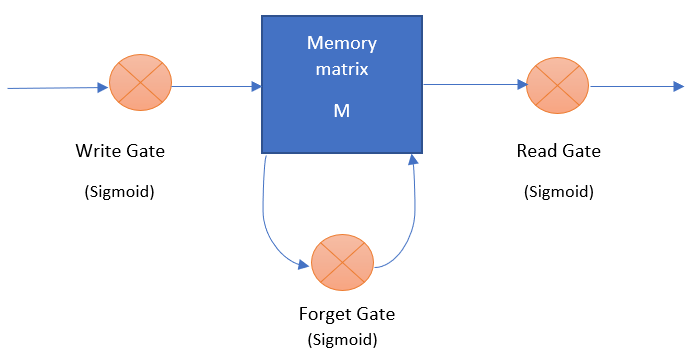
\includegraphics[width=0.5\textwidth]{3.PNG}
\caption{Model Architecture}
\label{fig:figure8}
\end{figure}

\subsection{Model Description} \label{Model description}
We have designed our system such that a separate recurrent neural network is being trained on each of the features extracted from a soloists repetoire. We then generate the feature using a starting seed and then recombine them to create a new solo. To achieve a fusion of different musical styles we have taken an approach wherein we generate the selected characteristis, notes, of a composition $A$, and a different characteristic, rhythm, of composition $B$ and so on. We then combine these features using a Generation Engine to recover a solo as shown in figure \ref{fig:figure9}

$$ Song_A = feature_A{1} + feature_A{2} + feature_A{3}$$
$$ Song_B = feature_B{1} + feature_B{2} + feature_B{3}$$
$$ Song_{Fusion} = feature_A{1} + feature_B{2} + feature_A{3}$$

We first pass the music files through a feature extraction engine as described in \ref{Preprocessing}. We then select the musical features that we are interested in combining from the music files. These features are then used to train the neural networks with a tunable memory parameter. Once trained these networks are used for generation of the learned features. These features are then passed through a Generation engine that works opposite to the Feature extraction, and combines the features to genrate a musical file.

\begin{figure}[h]
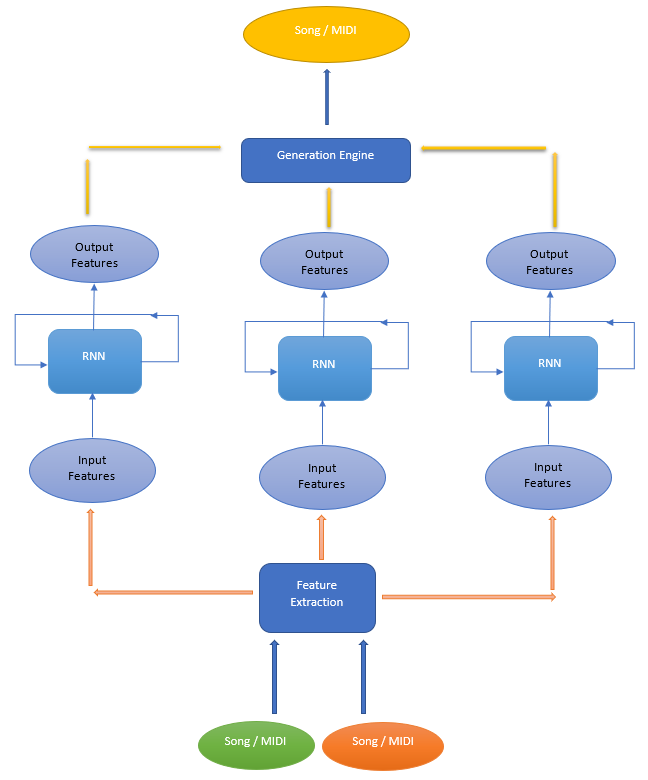
\includegraphics[width=0.5\textwidth]{IEEEtran/2.PNG}
\caption{System architecture}
\label{fig:figure9}
\end{figure}

\subsubsection{Model for Notes}
We train a LSTM recurrent neural network using the notes extracted from musical composition as described in \ref{f1pitch}. Here we use a sliding memory window of size $M$. We create training set by sliding the window over the entire interval and can be represented as follows:
$$feature = {note_{t},note_{t+1},...,note_{t+(M-1)}}$$
$$label = {note_{t+M}}$$

We generate similar feature-label pairs from the musical composition. Then we use a deep recurrent LSTM network with 256 nodes, one hidden layer, a dropout of 0.2 coupled with a \texttt{softmax} activation function. We use \texttt{categorical cross-entropy} as our loss function.\\

\begin{figure}[h]
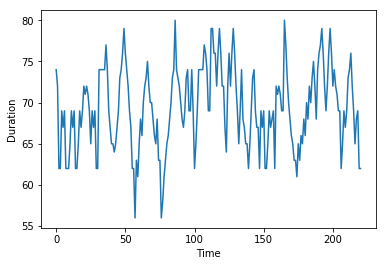
\includegraphics[width=0.5\textwidth]{IEEEtran/notes_o.png}
\caption{Time Variation of Original Notes}
\label{fig:figure1}
\end{figure}

\begin{figure}[h]
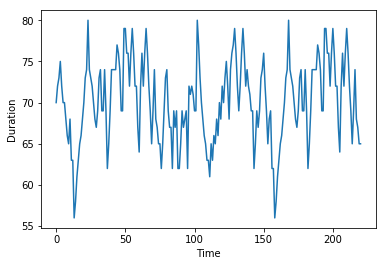
\includegraphics[width=0.5\textwidth]{IEEEtran/notes_g.png}
\caption{Time Variation of Generated Notes}
\label{fig:figure2}
\end{figure}

\subsubsection{Model for amplitude}
We train a LSTM recurrent neural network using the aplitudes extracted from musical composition as described in \ref{f2rhythm}. Here we use a sliding memory window of size $M$. We create training set by sliding the window over the entire interval and can be represented as follows:
$$feature = {amplitude_{t},amplitude_{t+1},...,amplitude_{t+(M-1)}}$$
$$label = {amplitude_{t+M}}$$

We generate similar feature-label pairs from the musical composition. Then we use a deep recurrent LSTM network with 256 nodes, one hidden layer, a dropout of 0.2 coupled with a \texttt{softmax} activation function. We use \texttt{categorical cross-entropy} as our loss function.\\

\begin{figure}[h]
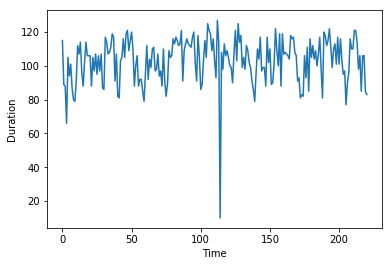
\includegraphics[width=0.5\textwidth]{IEEEtran/amp_o.png}
\caption{Time Variation of Original Amplitudes}
\label{fig:figure3}
\end{figure}

\begin{figure}[h]
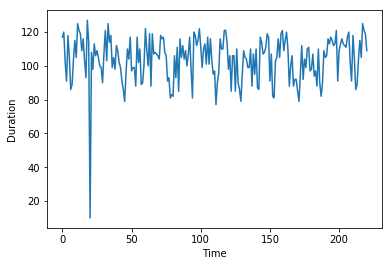
\includegraphics[width=0.5\textwidth]{IEEEtran/amp_g.png}
\caption{Time Variation of Generated Amplitudes}
\label{fig:figure4}
\end{figure}

\subsubsection{Model for Velocities}
We train a LSTM recurrent neural network using the velocities extracted from musical solo as described in \ref{f1pitch}. Here we use a sliding memory window of size $M$. We create training set by sliding the window over the entire interval and can be represented as follows:
$$feature = {velocity_{t},velocity_{t+1},.....velocity_{t+(M-1)}}$$
$$label = {velocity_{t+M}}$$

We generate similar feature-label pairs from the musical composition. Then we use a recurrent LSTM network with 4 nodes. We use \texttt{mean squared error} as our loss function.
\begin{figure}[h]
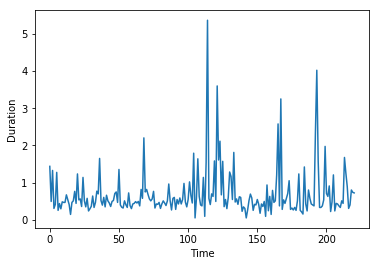
\includegraphics[width=0.5\textwidth]{IEEEtran/rest_o.png}
\caption{Time Variation of Original Velocity}
\label{fig:figure5}
\end{figure}

\begin{figure}[h]
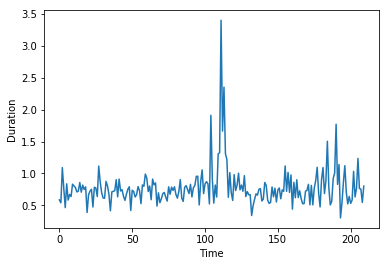
\includegraphics[width=0.5\textwidth]{IEEEtran/rest_g.png}
\caption{Time Variation of Generated Velocity}
\label{fig:figure6}
\end{figure}
% An example of a floating figure using the graphicx package.
% Note that \label must occur AFTER (or within) \caption.
% For figures, \caption should occur after the \includegraphics.
% Note that IEEEtran v1.7 and later has special internal code that
% is designed to preserve the operation of \label within \caption
% even when the captionsoff option is in effect. However, because
% of issues like this, it may be the safest practice to put all your
% \label just after \caption rather than within \caption{}.
%
% Reminder: the "draftcls" or "draftclsnofoot", not "draft", class
% option should be used if it is desired that the figures are to be
% displayed while in draft mode.
%
%\begin{figure}[!t]
%\centering
%\includegraphics[width=2.5in]{myfigure}
% where an .eps filename suffix will be assumed under latex,
% and a .pdf suffix will be assumed for pdflatex; or what has been declared
% via \DeclareGraphicsExtensions.
%\caption{Simulation results for the network.}
%\label{fig_sim}
%\end{figure}

% Note that the IEEE typically puts floats only at the top, even when this
% results in a large percentage of a column being occupied by floats.


% An example of a double column floating figure using two subfigures.
% (The subfig.sty package must be loaded for this to work.)
% The subfigure \label commands are set within each subfloat command,
% and the \label for the overall figure must come after \caption.
% \hfil is used as a separator to get equal spacing.
% Watch out that the combined width of all the subfigures on a
% line do not exceed the text width or a line break will occur.
%
%\begin{figure*}[!t]
%\centering
%\subfloat[Case I]{\includegraphics[width=2.5in]{box}%
%\label{fig_first_case}}
%\hfil
%\subfloat[Case II]{\includegraphics[width=2.5in]{box}%
%\label{fig_second_case}}
%\caption{Simulation results for the network.}
%\label{fig_sim}
%\end{figure*}
%
% Note that often IEEE papers with subfigures do not employ subfigure
% captions (using the optional argument to \subfloat[]), but instead will
% reference/describe all of them (a), (b), etc., within the main caption.
% Be aware that for subfig.sty to generate the (a), (b), etc., subfigure
% labels, the optional argument to \subfloat must be present. If a
% subcaption is not desired, just leave its contents blank,
% e.g., \subfloat[].


% An example of a floating table. Note that, for IEEE style tables, the
% \caption command should come BEFORE the table and, given that table
% captions serve much like titles, are usually capitalized except for words
% such as a, an, and, as, at, but, by, for, in, nor, of, on, or, the, to
% and up, which are usually not capitalized unless they are the first or
% last word of the caption. Table text will default to \footnotesize as
% the IEEE normally uses this smaller font for tables.
% The \label must come after \caption as always.
%
%\begin{table}[!t]
%% increase table row spacing, adjust to taste
%\renewcommand{\arraystretch}{1.3}
% if using array.sty, it might be a good idea to tweak the value of
% \extrarowheight as needed to properly center the text within the cells
%\caption{An Example of a Table}
%\label{table_example}
%\centering
%% Some packages, such as MDW tools, offer better commands for making tables
%% than the plain LaTeX2e tabular which is used here.
%\begin{tabular}{|c||c|}
%\hline
%One & Two\\
%\hline
%Three & Four\\
%\hline
%\end{tabular}
%\end{table}


% Note that the IEEE does not put floats in the very first column
% - or typically anywhere on the first page for that matter. Also,
% in-text middle ("here") positioning is typically not used, but it
% is allowed and encouraged for Computer Society conferences (but
% not Computer Society journals). Most IEEE journals/conferences use
% top floats exclusively.
% Note that, LaTeX2e, unlike IEEE journals/conferences, places
% footnotes above bottom floats. This can be corrected via the
% \fnbelowfloat command of the stfloats package.


\section{Experiments \& Results}
We experimented the with learning the features of a musical composition as described in \ref{Feature Engineering} above. We have mainly utilized Keras \cite{keras} for training the neural networks.

\section{Future Scope}
We have restricted our work to use of three features described in section \ref{Feature Engineering}. In general a musical composition can be used to extract many features some of which are spectral centroid, high frequency energy, high frequency content, spectral irregularity, spectral flux and running entropy, vector-based bandpass filter envelopes are Fourier transform with a sliding window.\cite{Jensen} These features can be used to enhance the learning and generation process.\\

Attempts were also made to produce a quasi-time series set such that the sample values were the MIDI pitches, silence being -1, and each sample representing a point in time of the file. This had the advantage of encoding both the rhythmic and pitch information in the same set. However, using an LSTM on this yielded unusable results. Nonetheless, it is perhaps an avenue for future experiments.\\

\section{Conclusion}
The current work has demonstrated that recurrent neural networks (RNNs) in combination with long short term memory (LSTM) cells, has the capability to capture temporal dynamics of a musical composition. Although not precise reproduction but we achieved very similar reproduction of the certain features, when we seeded the network with beginning of time $t_0$ for a musical composition. Our motive in this paper was to focus on generative aspects of the musical composition so we seeded the network randomly which resulted in generation of different samples. The periodicity of feature patterns are preserved in such cases, but the the coordination information seems to be lost when we try recombination of the same.\\

\\This is in accordance with out expectations as we did not want an entire reproduction of the samples. We wanted the sensitivity of out network to be high, but also a good amount specificity so that the network could learn a generic style which can then be used in combination with counterpart features from fundamentally variant data points. Our experiments yielded good results where we just restricted the features to being notes, rest and amplitude as defined in the section.\ref{Feature Engineering} Although we would prefer keeping the model simple, we expect improved results by taking into account an increased number of uncorrelated features. On the basis of our experiments we can say that the technique presented here can definitely be used for fusion of different musical styles. We are eager to experiment with more complex architectures and variant styles to see how well out preliminary results evolve on tuning various parameters.


% conference papers do not normally have an appendix


% use section* for acknowledgment
%\section*{Acknowledgment}


%The authors would like to thank...





% trigger a \newpage just before the given reference
% number - used to balance the columns on the last page
% adjust value as needed - may need to be readjusted if
% the document is modified later
%\IEEEtriggeratref{8}
% The "triggered" command can be changed if desired:
%\IEEEtriggercmd{\enlargethispage{-5in}}

% references section

% can use a bibliography generated by BibTeX as a .bbl file
% BibTeX documentation can be easily obtained at:
% http://mirror.ctan.org/biblio/bibtex/contrib/doc/
% The IEEEtran BibTeX style support page is at:
% http://www.michaelshell.org/tex/ieeetran/bibtex/
%\bibliographystyle{IEEEtran}
% argument is your BibTeX string definitions and bibliography database(s)
%\bibliography{IEEEabrv,../bib/paper}
%
% <OR> manually copy in the resultant .bbl file
% set second argument of \begin to the number of references
% (used to reserve space for the reference number labels box)
\begin{thebibliography}{1}

\bibitem{lstm}
Hasim Sak, Andrew Senior, Francoise Beaufays, \emph{Long Short-Term Memory Recurrent Neural Network Architectures for Large Scale Acoustic Modeling}.\hskip 1em plus 0.5em minus 0.4em\relax Google, USA

\bibitem{sturm}
Bob L. Sturm, Joao Felipe Santos, Iryna Korshunova, \emph{Folk music style modelling by recurrent neural networks with long short term memory units}.\hskip 1em plus 0.5em minus 0.4em\relax Late-breaking demo at the 2015 Int. Symposium on Music Information Retrieval.

\bibitem{judy}
Judy A. Franklin. \emph{Recurrent neural networks for music computation}.\hskip 1em plus 0.5em minus 0.4em\relax ORSA journal on computing, 18(3):321–338, 2006

\bibitem{judy1}
Judy A. Franklin, Krystal K. Locke, \emph{Recurrent Neural Networks For Musical Pitch memory and classification}.\hskip 1em plus 0.5em minus 0.4em\relax International Journal on Artificial Intelligence Tools\relax. July, 2004

\bibitem{judy2}
Judy A. Franklin. \emph{Jazz Melody Generation from Recurrent Network Learning of Several Human Melodies}.\hskip 1em plus 0.5em minus 0.4em\relax American Association for Artificial Intelligence, 2005

\bibitem{todd}
Bharucha, J. J. and Todd, P. M. \emph{Modeling the perception of tonal structure with neural nets}. \hskip 1em plus 0.5em minus 0.4em\relax Computer Music Journal, \relax 13(4):44–53.(1989)

\bibitem{eck}
Douglas Eck, J\u{u}ergen Schmidhuber. \emph{A First Look at Music Composition using LSTM Recurrent Neural Networks}\hskip 1em plus 0.5em minus 0.4em\relax Instituto Dalle Molle di studi sull\' intelligenza artificiale Galleria 2 \relax Technical Report No. IDSIA-07-02

\bibitem{mozer}
Stevens, C. and Wiles, J. (1994).\emph{Representations of tonal music: A case study in the development of temporal relationship}. In Mozer, M., Smolensky, P., Touretsky, D., Elman, J., and Weigend, A. S., editors,\hskip 1em plus 0.5em minus 0.4em\relax Proceedings of the 1993 Connectionist Models Summer School,\relax pages 228–235.

\bibitem{hochreiter}
Hochreiter, S., Bengio, Y., Frasconi, P., and Schmidhuber, J. (2001). \emph{Gradient flow in recurrent nets: the difficulty of learning long-term dependencies}.\hskip 1em plus 0.5em minus 0.4em\relax In Kremer, S. C. and Kolen, J. F.,editors, A Field Guide to Dynamical Recurrent Neural Networks.\relax IEEE Press

\bibitem{keefe}
B.Laden and D.H.Keefe. \emph{The Representation of Pitch in a Neural Net Model of Chord Classification Music and Connectionism},\hskip 1em plus 0.5em minus 0.4em\relax eds. Todd, P.M. and Loy, E.D.,\relax (MIT Press, Cambridge, MA, 1991)

\bibitem{Jensen}
K. Jensen and T.H. Andersen. \emph{Real-time beat estimation using feature extraction},\hskip 1em plus 0.5em minus 0.4em\relax Jensen2003RealTimeBE \relax 2003


\bibitem{IEEEhowto:kopka}
H.~Kopka and P.~W. Daly, \emph{A Guide to \LaTeX}, 3rd~ed.\hskip 1em plus 0.5em minus 0.4em\relax Harlow, England: Addison-Wesley, 1999.

\bibitem{keras}
Chollet Fran\c{c}ois and others, \emph{Keras} \url{https://github.com/fchollet/keras} \relax 2015

\end{thebibliography}




% that's all folks
\end{document}
